\documentclass[12pt]{article}
\linespread{1}

% margins
\setlength{\textwidth}{6.5in}
\setlength{\textheight}{8.75in}
\setlength{\oddsidemargin}{-0.1in}
\setlength{\topmargin}{-0.1in}
\setlength{\baselineskip}{10pt}

% load packages
\usepackage{amsmath}
\usepackage{amsfonts}
\usepackage{lscape}
\usepackage[round]{natbib}
\usepackage{graphicx}
\graphicspath{{figures/}}
\usepackage{amssymb}
\usepackage{color}
\usepackage{hyperref}
\usepackage{booktabs}

% style setup
\bibliographystyle{plainnat}
\pagestyle{empty}
\setlength\parindent{0pt}
\setlength{\parskip}{\baselineskip}

% new commands
\newcommand{\indist}{\overset{d}{\rightarrow}}
\newcommand{\inprob}{\overset{P}{\rightarrow}}
\newcommand{\tabby}{\hspace{10pt}}
\newcommand{\ones}{{\bf 1}}
\newcommand{\tp}{\intercal}
\newcommand{\iprod}[2]{\langle #1 , #2 \rangle}

\newcommand{\note}[1]{\textcolor{red}{#1}}

% header
\title{HOSEA project updates}
\author{Peter MacDonald}
\date{\today}

\begin{document}

%\maketitle

\subsubsection*{04/13 update}

\begin{itemize}
  \item Preliminary results on a small, {\bf balanced} subsample (5000 cases, 5000 controls).
  \item Training set of 9000 IDs, test set of 1000 IDs.
  \item Imputed missing variables with median.
  \item Lab data (blood tests, FOBT) and colonoscopies converted to longitudinal summaries (mean,max,min,...).
  \item Lab data restricted to time interval from `indexdate - 3 years' to `indexdate - 1 year'.
  \item No ICD code information, no medication information, no smoking status records (smoking status at index is in demographic variables).
  \item Logistic regression.
\end{itemize}

\begin{center}
\begin{table}[h!!]
\begin{tabular}{|l|l|l|}
\hline
\textbf{Predictors ($p=$ \# of predictors)}                                                & \textbf{Training AUC} & \textbf{Test AUC} \\ \hline
Demographic ($p=10$)                                     & 0.814                 & 0.818             \\ \hline
Charlson ($p=18$)                                     & 0.705               & 0.693         \\ \hline
Demographic + Charlson ($p=28$)             & 0.863                 & 0.862             \\ \hline
Labs ($p=210$)                                                 & 0.824                 & 0.824             \\ \hline
Demographic + Charlson + Labs ($p=238$) & 0.913                 & 0.910             \\ \hline
\end{tabular}
\end{table}
\end{center}

\pagebreak

\subsubsection*{04/20 update}

\begin{itemize}
  \item Preliminary results on a small, {\bf balanced} subsample (5000 cases, 5000 controls).
  \item Training set of 9000 IDs, test set of 1000 IDs.
  \item Imputed missing variables with median.
  \item {\bf Sets of predictors:}
  \begin{itemize}
    \item Demographic data includes race, age, weight, etc. ({\bf Demographic}).
    \item Charlson score inputs plus GERD diagnosis ({\bf Charlson}).
    \item Lab data (blood tests, FOBT) and colonoscopy data converted to longitudinal summaries (mean,max,min,...) ({\bf Labs}).
    \item Medication (H2R and PPI) converted to longitudinal summaries (mean,max,...) ({\bf Meds}).
  \end{itemize}
  \item Lab and medication data restricted to time interval from `indexdate - 3 years' to `indexdate - 1 year'.
  \item Logistic regression.
\end{itemize}

\begin{center}
\begin{table}[h!!]
\begin{tabular}{|l|l|l|}
\hline
\textbf{Predictors ($p=$ \# of predictors)}                                                & \textbf{Training AUC} & \textbf{Test AUC} \\ \hline
Demographic ($p=10$)                                     & 0.814                 & 0.818             \\ \hline
Charlson ($p=18$) & 0.705 & 0.693                                                            \\ \hline
Meds ($p=10$)                                                 & 0.604              & 0.598       \\ \hline
Demographic + Charlson + Labs + Meds ($p=240$)                                                 & 0.915                & 0.912            \\ \hline
\end{tabular}
\end{table}
\end{center}

\pagebreak

\subsubsection*{04/27 update}

\begin{itemize}
  \item Baseline logistic regression on entire sample (no blood labs, no medication data).
  \item Full sample contains $n = 6,649,108$ observations, with $n_{\text{control}} = 6,637,713$ and \\ $n_{\text{case}} = 11,395$.
  %\item About 582 controls for every case.
  \item Imputed numeric variables with medians, imputed smoking status at random, proportional to non-missing in sample (45\% current, 41\% former, 14\% never).
\end{itemize}

\begin{center}
\begin{tabular}{|l|l|l|}
\hline
\textbf{Predictors ($p=$ \# of predictors)}                                                & \textbf{Training AUC} & \textbf{Test AUC} \\ \hline
Demographic ($p=10$)                                     & 0.670                & 0.675            \\ \hline
Charlson ($p=18$) & 0.684 & 0.705                                                          \\ \hline
Demographic + Charlson ($p=28$)                                                 & 0.760               & 0.770     \\ \hline
\end{tabular}
\end{center}
{\bf Smoking status missingness.}

In the entire sample:
\begin{center}
\begin{tabular}{|l|l|l|l|l|}
\hline
\textbf{Smoking Status} & Current & Former & Never & Missing \\ \hline
Count & 1696052 & 1521806 & 537727 & 2893523 \\ \hline
Probability & 0.26 & 0.23 & 0.08 & \note{0.44} \\ \hline
\end{tabular}
\end{center}

Among cases:
\begin{center}
\begin{tabular}{|l|l|l|l|l|}
\hline
\textbf{Smoking Status} & Current & Former & Never & Missing \\ \hline
Count & 3901 & 3546 & 594 & 3354 \\ \hline
Probability & 0.34 & 0.31 & 0.05 & \note{0.29} \\ \hline
\end{tabular}
\end{center}

Among controls:
\begin{center}
\begin{tabular}{|l|l|l|l|l|}
\hline
\textbf{Smoking Status} & Current & Former & Never & Missing \\ \hline
Count & 1692151 & 1518260 & 537133 & 2890169 \\ \hline
Probability & 0.25 & 0.23 & 0.08 & \note{0.44} \\ \hline
\end{tabular}
\end{center}

\pagebreak

\subsubsection*{05/04 update}
\begin{itemize}
  \item Preliminary results on a balanced {\bf random sample} of 5000 cases and 5000 controls.
  \item Most missing variables imputed with their median, SmokeStatus imputed at random proportional to non-missing. %(about 45/41/14\% current/former/never)
  \item Training on 9000 observations, testing on 1000 observations.
  \item Baseline logistic regression fit with subsets of predictors, and all predictors.
  \item Random forest fit with all predictors.
\end{itemize}
\begin{center}
\begin{tabular}{|l|l|l|}
\hline
\textbf{Model/predictors ($p=$ \# of predictors)} & \textbf{Training AUC} & \textbf{Test AUC} \\ \hline
{\bf Logistic regression} & - & - \\ \hline
Demographic ($p=10$) & 0.669 & 0.676 \\ \hline
Charlson ($p=18$) & 0.689 & 0.659 \\ \hline
Meds ($p=10$) & 0.515 & 0.513 \\ \hline
Colonoscopies ($p=2$) & 0.513 & 0.502 \\ \hline
Labs ($p=200$) & 0.671 & 0.621 \\ \hline
All ($p=240$) & {\bf 0.814} & {\bf 0.778} \\ \hline
{\bf Random forest} & - & - \\ \hline
All ($p=240$) & {\bf 0.985} & {\bf 0.844} \\ \hline
\end{tabular}
\end{center}
{\bf Random forest variable importance.}
Most important blood lab measurements (all means of measurements over the 2 year window):
\begin{enumerate}
  \item Hematocrit value (CBC labs)
  \item MCH value (CBC labs)
  \item ALT value (LFT labs)
  \item Alk. Phos. value (LFT labs)
  \item AST value (LFT labs)
  \item White blood cells (WBC) value (CBC labs)
  \item Glucose value (BMP labs)
\end{enumerate}
{\bf Next steps:}
\begin{itemize}
  \item Better approaches to impute missing variables (esp. SmokeStatus).
  \item Improved non-linear classifiers for subsample.
  \item Logistic regression baselines for the full sample of 6M observations.
\end{itemize}

\pagebreak

\subsubsection*{05/11 update}
\begin{itemize}
  \item Baseline logistic regression on full sample (no medication data).
  \item $n = 6,649,108$ observations, with $n_{\text{control}} = 6,637,713$ and $n_{\text{case}} = 11,395$.
  %\item About 582 controls for every case.
  \item Most missing variables imputed with their median, SmokeStatus imputed at random proportional to non-missing.
  \item For lab information, only means of each measurement, no longitudinal information so far.
  \item \note{05/27 update:} Charlson and Demographic+Charlson updated to exclude Cancer and Metastatic Carcinoma.
\end{itemize}
\begin{center}
\begin{tabular}{|l|l|l|}
\hline
\textbf{Model/predictors ($p=$ \# of predictors)} & \textbf{Training AUC} & \textbf{Test AUC} \\ \hline
Demographic ($p=10$) & 0.670 & 0.675 \\ \hline
Charlson (\note{$p=16$}) & \note{0.684} & \note{0.705} \\ \hline
Demographic + Charlson (\note{$p=26$})                                                 & \note{0.760}               & \note{0.770}     \\ \hline
Colonoscopies ($p=2$) & 0.511 & 0.504 \\ \hline
Labs ($p=34$) & 0.604 & 0.601 \\ \hline
\note{Meds ($p=10$)} & \note{0.523} & \note{0.512} \\ \hline
%All ($p=64$) & {\bf 0.814} & {\bf 0.778} \\ \hline
\end{tabular}
\end{center}
{\bf Next steps:}
\begin{itemize}
  \item Process medication data.
  \item Approaches to impute missing variables (esp. SmokeStatus).
  \item Non-linear classifiers for subsample, plots/graphics to interpret predictor effects.
\end{itemize}

\pagebreak

\subsubsection*{05/18 update}

\begin{itemize}
  \item Medication data processed for full sample, new line (\note{red}) added to last week's table of baseline logistic regression AUCs.
  \item Gradient boosting implemented for the random sample of 5000 cases and 5000 controls.
\end{itemize}
\begin{center}
\begin{tabular}{|l|l|l|}
\hline
\textbf{Model/predictors ($p=$ \# of predictors)} & \textbf{Training AUC} & \textbf{Test AUC} \\ \hline
{\bf Logistic regression} & - & - \\ \hline
All ($p=240$) & 0.814 & 0.778 \\ \hline
{\bf Random forest} & - & - \\ \hline
All ($p=240$) & {\bf 0.985} & 0.844 \\ \hline
{\bf Gradient boosting} & - & - \\ \hline
All ($p=240$), no interactions & 0.900 & 0.847 \\ \hline
All ($p=240$), 2-way interactions & 0.924 & 0.857 \\ \hline
All ($p=240$), 3-way interactions & 0.937 & {\bf 0.864} \\ \hline
\end{tabular}
\end{center}
Same gradient boosting results without Charlson score inputs or GERD at index:
\begin{center}
\begin{tabular}{|l|l|l|}
\hline
\textbf{Model/predictors ($p=$ \# of predictors)} & \textbf{Training AUC} & \textbf{Test AUC} \\ \hline
{\bf Gradient boosting} & - & - \\ \hline
No Charlson inputs ($p=222$), no interactions & 0.881 & 0.811 \\ \hline
No Charlson inputs ($p=222$), 2-way interactions & 0.898 & 0.820 \\ \hline
No Charlson inputs ($p=222$), 3-way interactions & 0.909 & 0.817 \\ \hline
\end{tabular}
\end{center}

{\bf Next steps}
\begin{itemize}
  \item Scaling up gradient boosting, dealing with unbalanced classes in full sample.
  \item Plots/graphics to interpret black box models.
\end{itemize}

\pagebreak

\subsubsection*{05/25 update}

\begin{itemize}
  \item Results now without Cancer and Metastatic Carcinoma inputs to Charlson score.
  \item Implemented scalable \texttt{xgboost} model, test AUC \textbf{0.860}.
\end{itemize}

\textbf{Partial dependence plots} (from xgboost model).
Demographic variables:
\begin{center}
\begin{tabular}{cc}
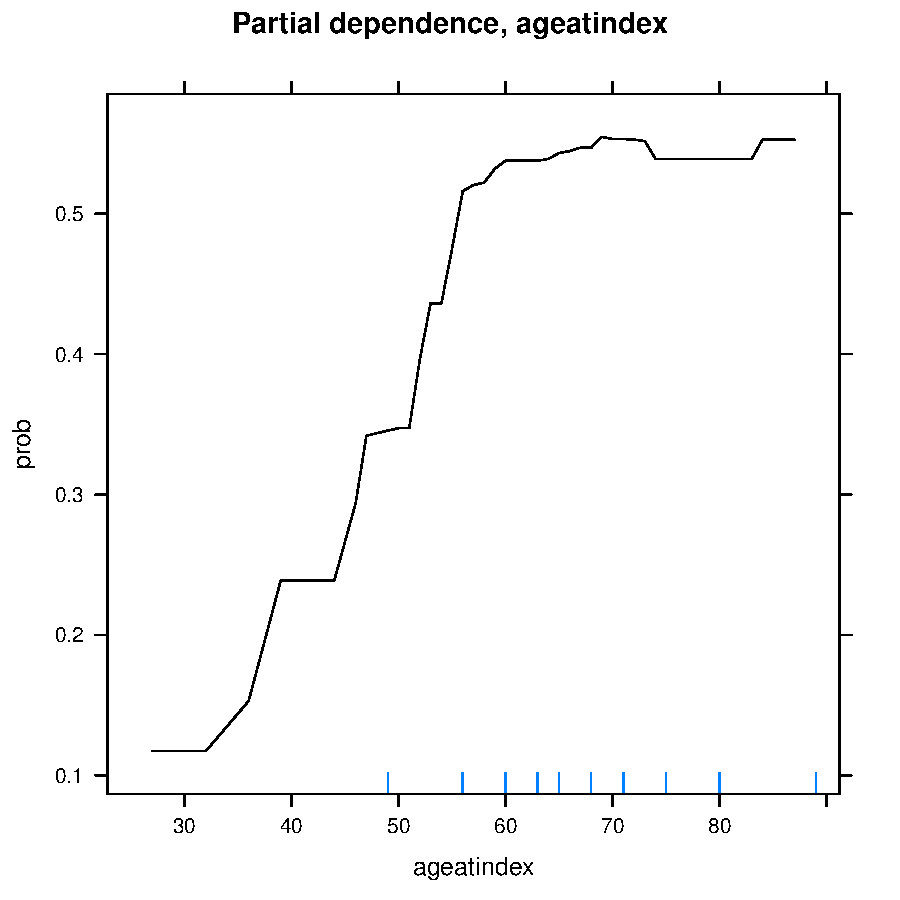
\includegraphics[width=.4\textwidth]{pdp_age.pdf} &
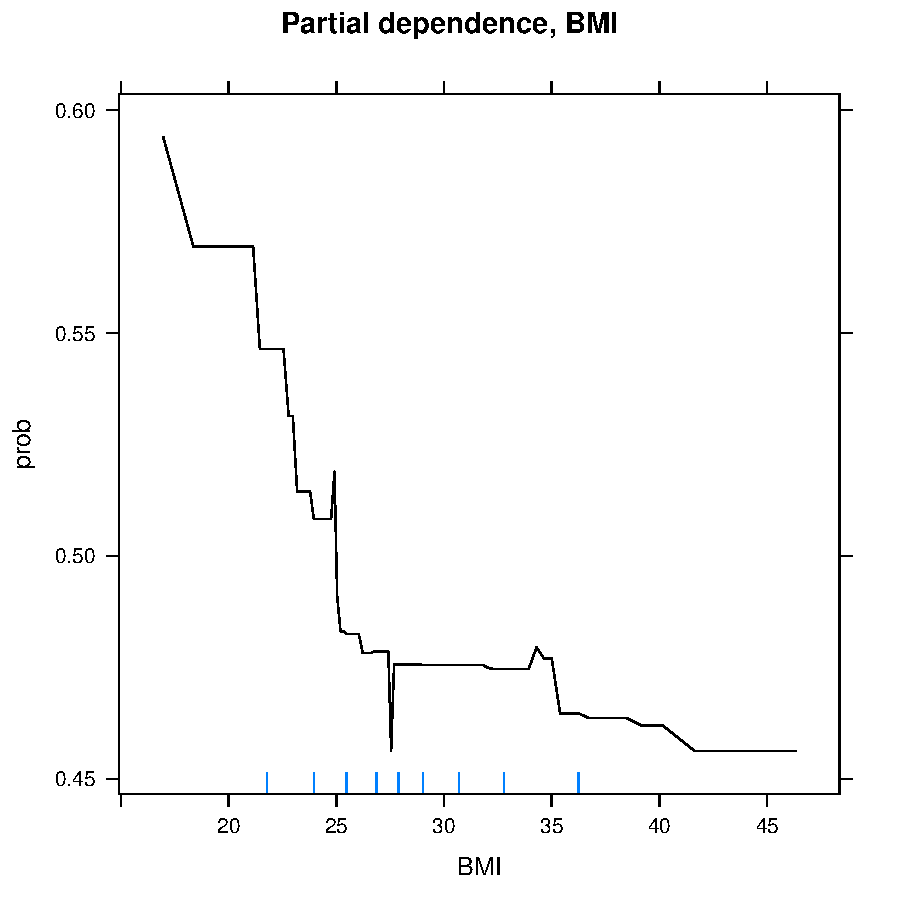
\includegraphics[width=.4\textwidth]{pdp_bmi.pdf} \\
\end{tabular}
\end{center}
Most influential blood lab variables:
\begin{center}
\begin{tabular}{cc}
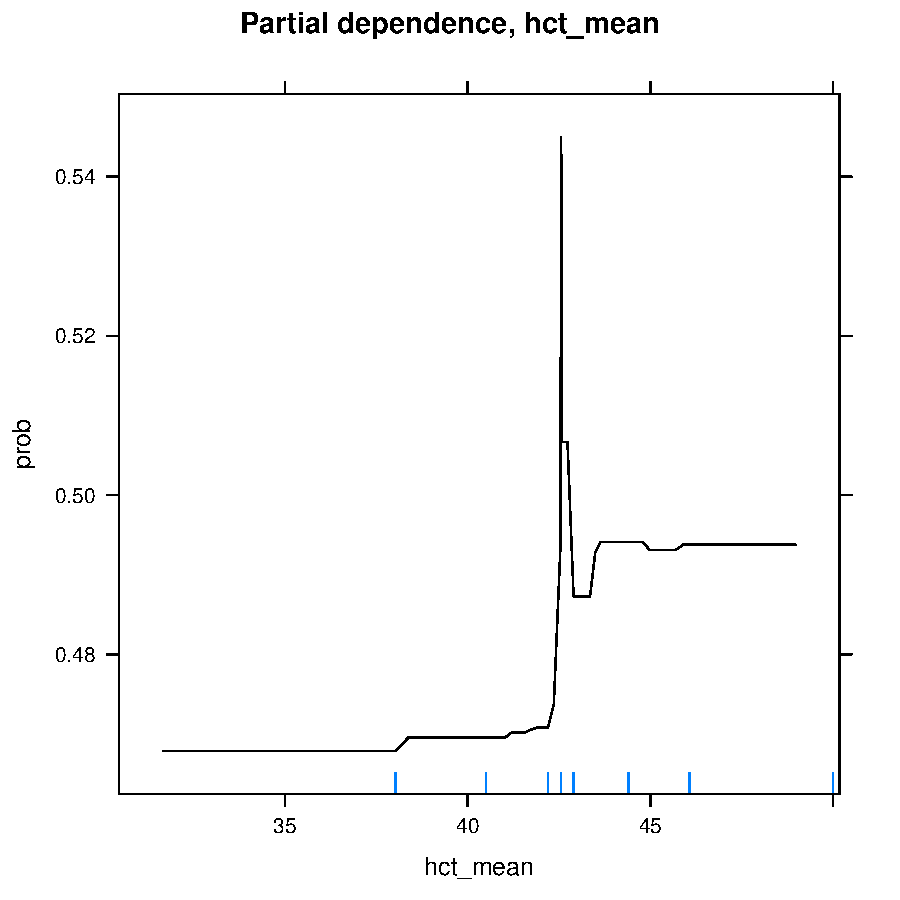
\includegraphics[width=.3\textwidth]{pdp_hct.pdf} &
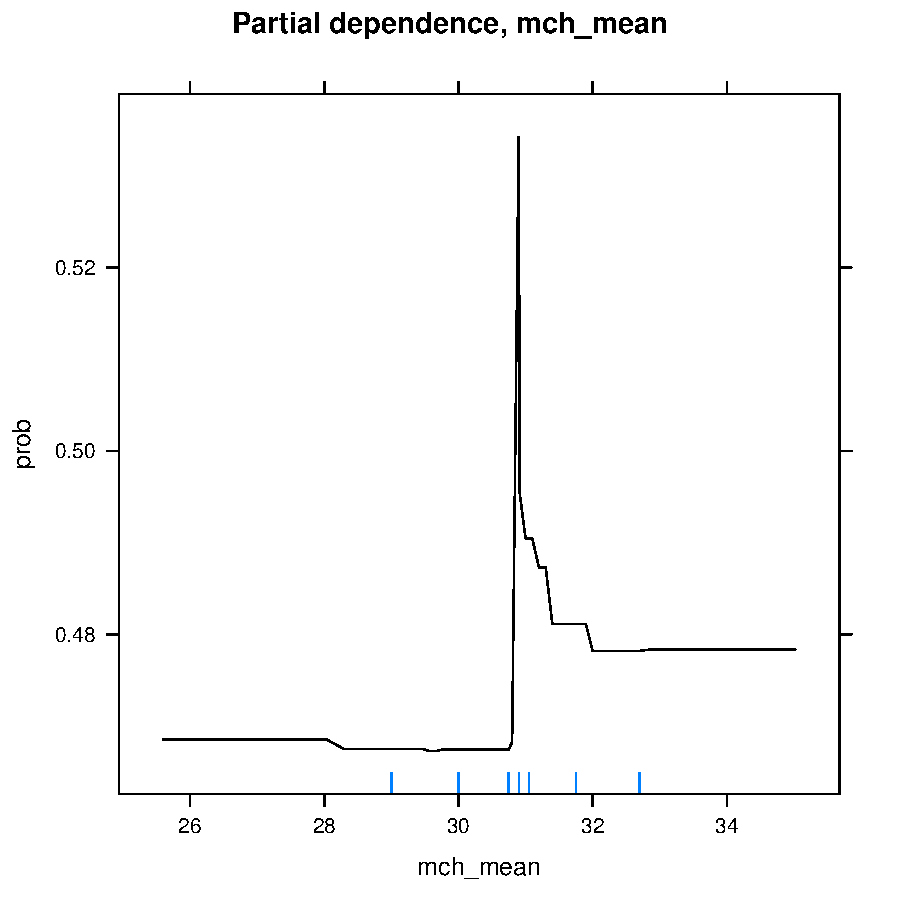
\includegraphics[width=.3\textwidth]{pdp_mch.pdf} \\
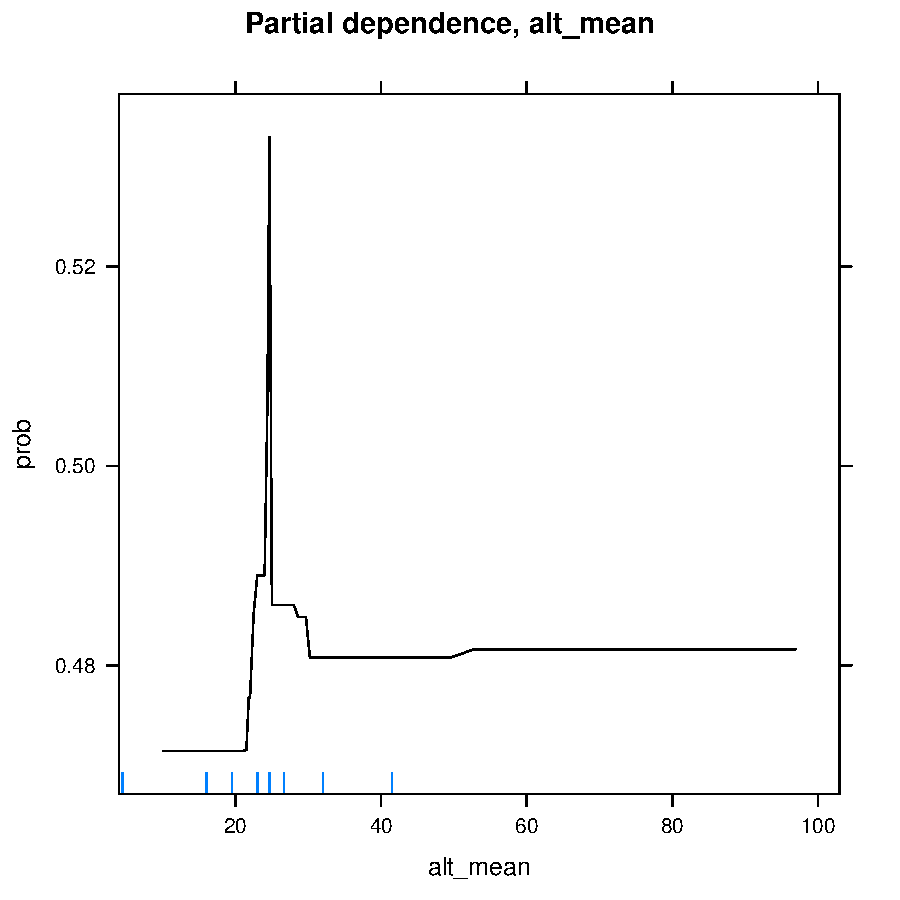
\includegraphics[width=.3\textwidth]{pdp_alt.pdf} &
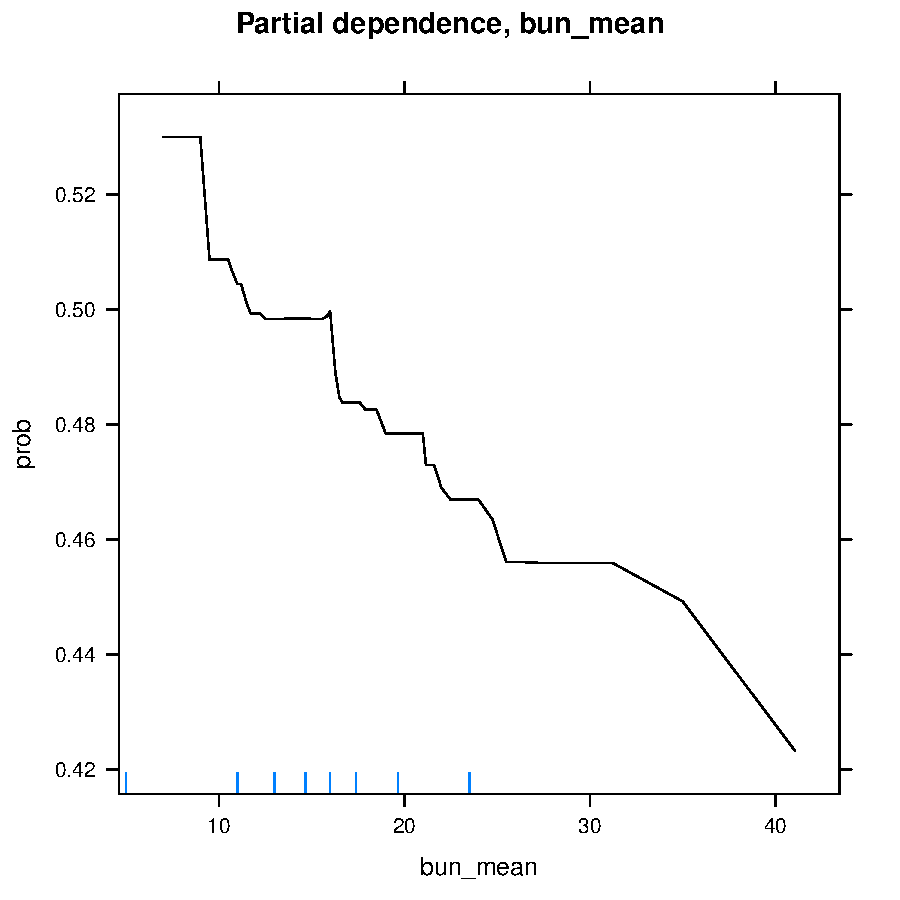
\includegraphics[width=.3\textwidth]{pdp_bun.pdf} \\
\end{tabular}
\end{center}

\textbf{Missingness rates for blood lab variables} (where `missing' means zero measurements of that variable in the 2 year window):
\begin{center}
\begin{tabular}{|l|l|l|}
\hline
\textbf{Proportion missing} & controls & cases \\ \hline
A1c\_mean (A1C Labs) & 0.51 & 0.52 \\ \hline
bun\_mean (BMP Labs) & 0.17 & 0.30 \\ \hline
hct\_mean (CBC Labs) & 0.20 & 0.50 \\ \hline
CRP\_mean (CRP Labs) & 0.95 & 0.94 \\ \hline
alkphos\_mean (LFT Labs) & 0.23 & 0.47 \\ \hline
chol\_mean (Lipid Labs) & 0.19 & 0.32 \\ \hline
\end{tabular}
\end{center}
\note{08/20: now with the new data, 4 year window from index-1 to index-5}
\begin{center}
\begin{tabular}{|l|l|l|}
\hline
\textbf{Proportion missing} & controls & cases \\ \hline
A1c\_mean (A1C Labs) & 0.43 & 0.47 \\ \hline
bun\_mean (BMP Labs) & 0.11 & 0.26 \\ \hline
hct\_mean (CBC Labs) & 0.12 & 0.46 \\ \hline
CRP\_mean (CRP Labs) & 0.93 & 0.91 \\ \hline
alkphos\_mean (LFT Labs) & 0.15 & 0.42 \\ \hline
chol\_mean (Lipid Labs) & 0.12 & 0.29 \\ \hline
\end{tabular}
\end{center}
\note{uniformly fewer missing, but rates are not cut in half, moreover heterogeneity of missingness between cases and controls is not fixed.}

\pagebreak

\subsubsection*{06/08 update}

\begin{itemize}
  \item Re-coded BMI/weight measurements?
  \item Re-run xgboost on balanced subsample with \texttt{NA}s, test AUC \textbf{0.880}, but it is using missing values to identify cases.
  \item Source of missingness? More detailed breakdown for LFT Labs.
\end{itemize}

\textbf{Updated partial dependence plots for blood lab variables.} Using new xgboost model on subsample.
\begin{center}
\begin{tabular}{cc}
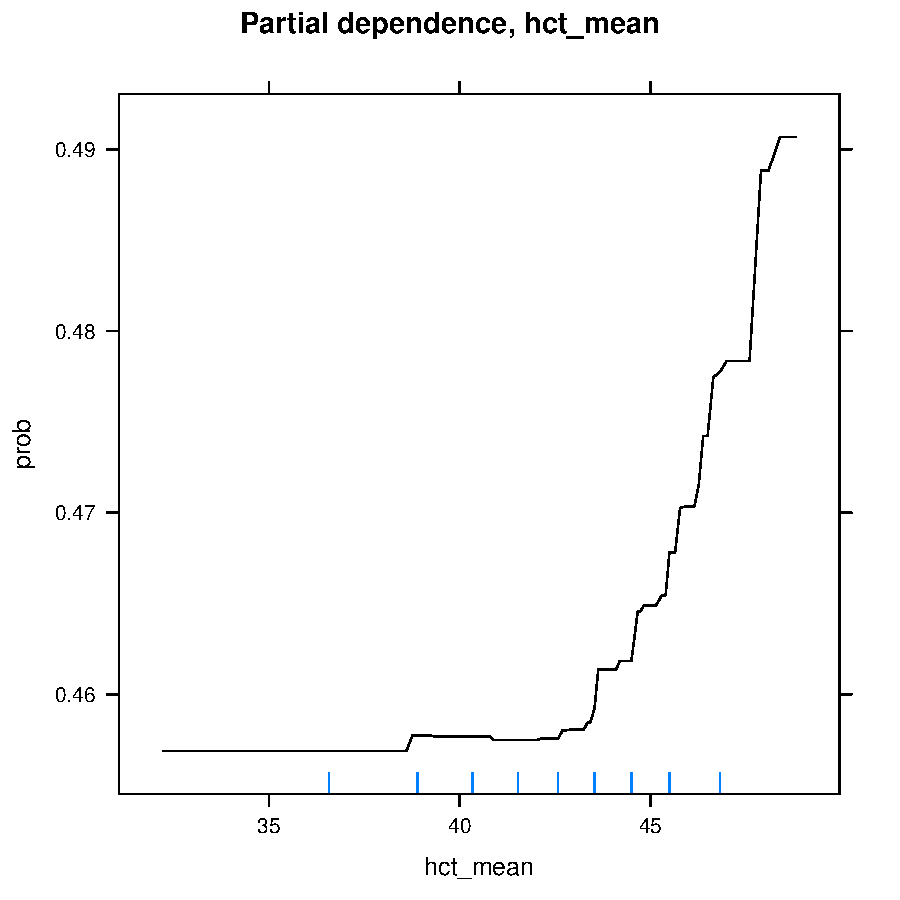
\includegraphics[width=.4\textwidth]{pdp_hct2.pdf} &
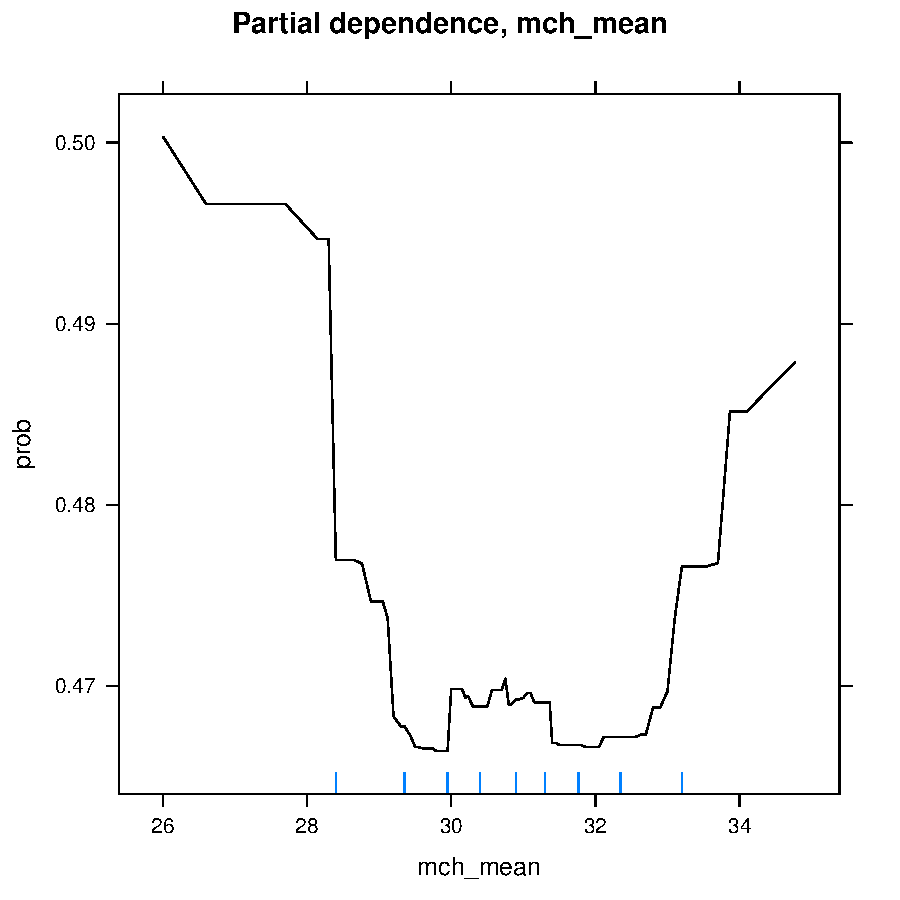
\includegraphics[width=.4\textwidth]{pdp_mch2.pdf} \\
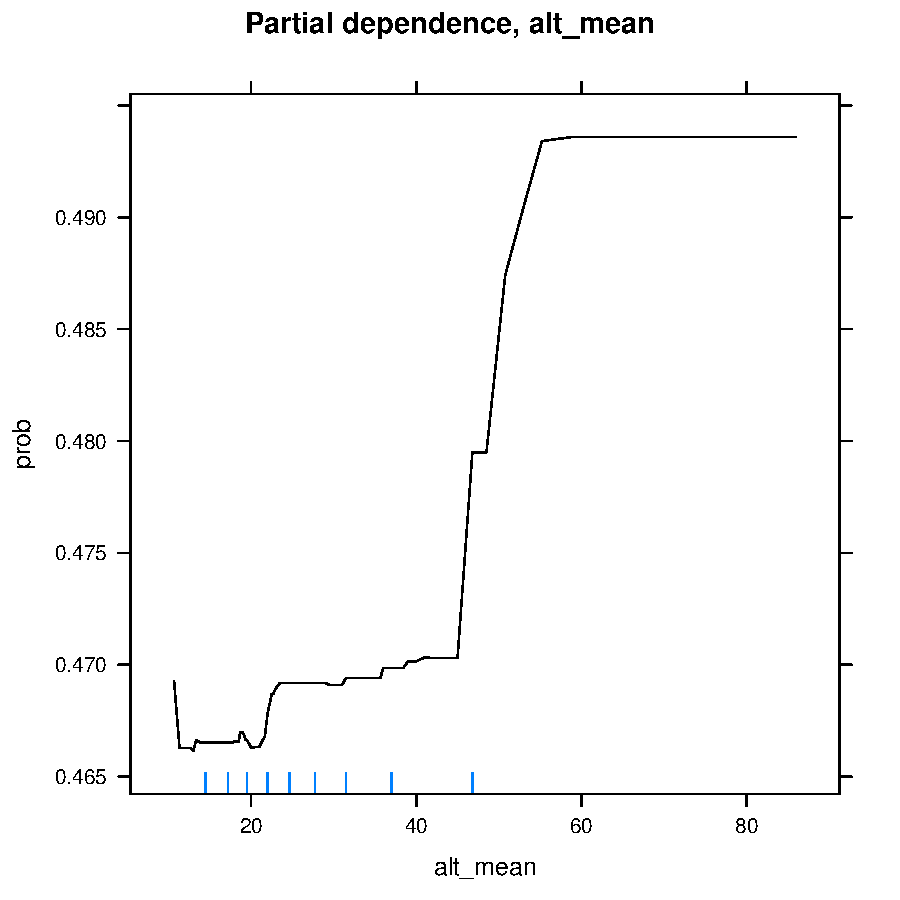
\includegraphics[width=.4\textwidth]{pdp_alt2.pdf} &
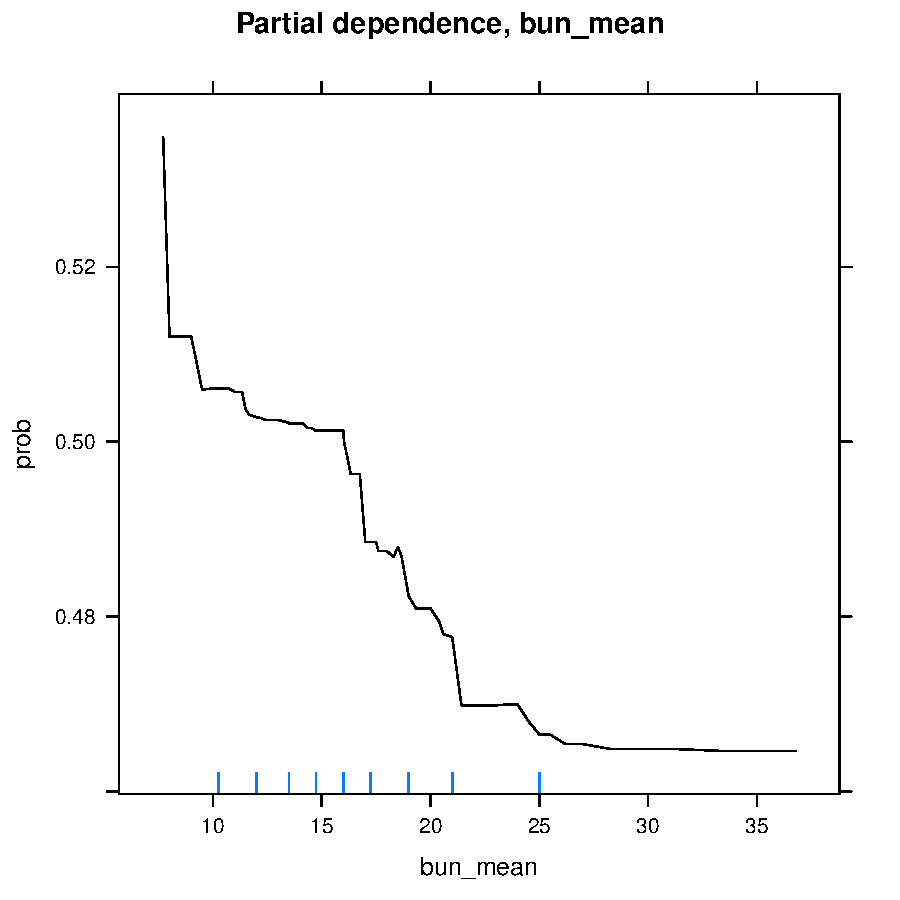
\includegraphics[width=.4\textwidth]{pdp_bun2.pdf} \\
\end{tabular}
\end{center}

\pagebreak

\textbf{Detailed breakdown of missingness for LFT labs.} (Prediction window is second and third years before index)
\begin{center}
\begin{tabular}{|l|l|l|}
\hline
\textbf{Mean \# of labs} & controls & cases \\ \hline
First year before index & 1.87 & 2.42 \\ \hline
Second year before index & 1.47 & 1.52 \\ \hline
Third year before index & 1.42 & 1.34 \\ \hline
\end{tabular}
\end{center}
Detailed breakdown for the prediction window (index minus 3 years to index minus 1 year):
\begin{center}
\begin{tabular}{|l|l|l|}
\hline
\textbf{Proportion} & controls & cases \\ \hline
At least 1 lab & 0.83 & 0.69 \\ \hline
At least 2 labs & 0.67 & 0.59 \\ \hline
At least 3 labs & 0.45 & 0.44 \\ \hline
At least 4 labs & 0.30 & 0.31 \\ \hline
At least 5 labs & 0.18 & 0.21 \\ \hline
\end{tabular}
\end{center}

\textbf{Next Steps:}
\begin{itemize}
  \item Imputation with xgboost
  \item Implement xgboost for entire sample
\end{itemize}

\pagebreak

\subsubsection*{06/22 update}

\begin{itemize}
  \item Set up code on GitLab (waljee-zhu-ml-projects/hosea-project).
  \item Received updated sample with recoded BMIs. BMIs are more likely to be missing for cases (14\%) than controls (8\%).
  \item Continuing to code imputation following Deng and Lumley (2021).
\end{itemize}

BMI comparison on the original sample data:
\begin{center}
\begin{tabular}{|l|l|l|l|l|l|l|}
\hline
 \textbf{Original BMI} & $< 20$ & $\in (20,25]$ & $\in (25,30]$ & $\in (30,35]$ & $\in (35,40]$ & $> 40$  \\ \hline
$\mathbb{P}(Control | BMI)$ & 0.9960 & 0.9978 & 0.9985 & 0.9985 & 0.9986 & 0.9986 \\ \hline
$\mathbb{P}(Case | BMI)$ & 0.0040 & 0.0022 & 0.0015 & 0.0015 & 0.0014 & 0.0014 \\ \hline
\end{tabular}
\end{center}

With the re-coded sample data:
\begin{center}
\begin{tabular}{|l|l|l|l|l|l|l|}
\hline
 \textbf{New BMI} & $< 20$ & $\in (20,25]$ & $\in (25,30]$ & $\in (30,35]$ & $\in (35,40]$ & $> 40$  \\ \hline
$\mathbb{P}(Control | BMI)$ & 0.9983 & 0.9985 & 0.9985 & 0.9984 & 0.9981 & 0.9979 \\ \hline
$\mathbb{P}(Case | BMI)$ & 0.0017 & 0.0015 & 0.0015 & 0.0016 & 0.0019 & 0.0021 \\ \hline
\end{tabular}
\end{center}

\pagebreak

\subsubsection*{06/29 update}

\begin{itemize}
  \item Now using updated data (new BMIs, Charlson scores).
  %\item Can bring back CANCER and MET\_CAR as predictors after re-processing?
  %\item Logistic regression is ``cheating'' with median imputation, using highly different missingess rates for Charlson scores
  \item For subsample, comparison of baseline logistic regression and xgboost models for different imputation approaches:
  \begin{enumerate}
    \item \textbf{No imputation}: leave NAs in the data, learn a classification for subjects with missing data (only compatible with xgboost).
    \item \textbf{Median imputation}: impute all variables with median/most common class.
    \item \textbf{Regression imputation}: impute by (linear) regression of each predictor variable on the others (similar to MICE).
    \item \textbf{Random sample imputation}: impute each predictor by sampling at random from the non-missing entries.
  \end{enumerate}
\end{itemize}

AUC results for xgboost/logistic regression for different imputation approaches. Results still on balanced subsample.
\begin{center}
\begin{tabular}{|l|l|l|l|}
\hline
\textbf{Imputation method/model} & \textbf{Training AUC} & \textbf{Test AUC} & \note{\textbf{Test AUC (complete records)}} \\ \hline
{\bf No imputation} & - & - & - \\ \hline
xgboost & 0.977 & 0.942 & \note{0.643} \\ \hline
{\bf Median imputation} & - & - & - \\ \hline
logistic regression & 0.834 & 0.810 & \note{0.585} \\ \hline
xgboost & 0.970 & 0.857 & \note{0.623} \\ \hline
{\bf Regression imputation} & - & - & - \\ \hline
logistic regression & 0.805 & 0.760 & \note{0.557} \\ \hline
xgboost & 0.948 & 0.815 & \note{0.705} \\ \hline
{\bf Random sample imputation} & - & - & - \\ \hline
logistic regression & 0.724 & 0.689 & \note{0.724} \\ \hline
xgboost & 0.919 & 0.729 & \note{\textbf{0.745}} \\ \hline
\end{tabular}
\end{center}

Regression imputation still has `regression to mean' effect for imputed values, imputed values have smaller variance than the true values (with observation error). Maybe try a version that imputes a rank then resamples from observed values.

% \textbf{Example:} Peptic Ulcer Disease (PUD) indicator.
%
% Among non-missing cases, 6.2\% have PUD=1. Among non-missing controls, 2.7\% have PUD=1.
%
% About 85\% of cases are missing PUD indicator, while about 47\% of controls are missing PUD indicator.
%
% After median imputation (PUD=NA becomes PUD=0 for all missing entries), 0.9\% of cases have PUD=1, 1.4\% of controls have PUD=1.

\pagebreak

\subsubsection*{07/06 update}

\begin{itemize}
  \item Source of missingness in the data? About 85\% of cases missing Charlson score inputs (compared to about 47\% of controls).
  \item Missingness in test set/use case?
  \item Updated \note{(in red)} last weeks results with a test set of 1000 complete records (226 cases, 774 controls).
  \begin{itemize}
    \item Poor generalization to complete cases for no imputation, median imputation implies that those models are fitting to the missingness, patterns won't continue to hold with fully observed data.
    \item Regression imputation still has `regression to mean' effect for imputed values, imputed values have smaller variance than the observed values (observation error).
    \item Good generalization of random sample imputation implies that there is no bias introduced from training on data with missingness.
  \end{itemize}
  %\item Memory issues fitting xgboost on the full data, will need to do some kind of batch training to handle the entire data.
\end{itemize}

\pagebreak

\subsubsection*{07/13 update}

\begin{itemize}
  \item Should we evaluate the model on complete records or missing/imputed records?
  \item Recall: previous results with an additional test set of 1000 complete records (226 cases, 774 controls).
  \begin{itemize}
    \item New comparison for \textbf{multiple} random sample imputation: imputes by sampling from non-missing entries several times (reps) for each missing value, training on the multiple imputed records.
    %\item Poor generalization to complete cases for no imputation, median imputation implies that those models are fitting to the missingness, patterns won't continue to hold with fully observed data.
    %\item Good generalization of random sample imputation implies that there is no bias introduced from training on data with missingness.
  \end{itemize}
  \item Memory issues fitting xgboost on the full data, implementing ``batched'' training.
\end{itemize}

AUC's for xgboost/logistic regression for different imputation approaches. Results still on balanced subsample.
\begin{center}
\begin{tabular}{|l|l|l|l|}
\hline
\textbf{Imputation method/} & \textbf{Training AUC} & \textbf{Test AUC} & \textbf{Test AUC} \\
\textbf{prediction model}& & \textbf{(imputed records)} & \textbf{(complete records)} \\ \hline
{\bf No imputation} & - & - & - \\ \hline
xgboost & 0.977 & 0.942 & 0.643 \\ \hline
{\bf Median imputation} & - & - & - \\ \hline
logistic regression & 0.834 & 0.810 & 0.585 \\ \hline
xgboost & 0.970 & 0.857 & 0.623 \\ \hline
{\bf Regression imputation} & - & - & - \\ \hline
logistic regression & 0.805 & 0.760 & 0.557 \\ \hline
xgboost & 0.948 & 0.815 & 0.705 \\ \hline
{\bf Random sample imputation} & - & - & - \\ \hline
logistic regression & 0.724 & 0.689 & 0.724 \\ \hline
xgboost & 0.919 & 0.729 & 0.745 \\ \hline
{\bf Multiple rand. samp.} & - & - & - \\ \hline
xgboost, 10 reps & 0.909 & 0.742 & 0.781 \\ \hline
xgboost, 20 reps & 0.939 & 0.765 & 0.820 \\ \hline
xgboost, 30 reps & 0.948 & 0.768 & 0.781 \\ \hline
\end{tabular}
\end{center}

Final two columns suggest two different evaluation metrics, ensuring the model performs well on \textbf{both} (A) new patients with imputed data and (B) new patients with fully observed blood labs, etc.

\pagebreak

\subsubsection*{07/20 update}

\begin{itemize}
  \item Continuing to test/tune imputation approaches.
  \item Notes on decision curve analysis.
\end{itemize}

\begin{center}
\begin{tabular}{|l|l|l|l|}
\hline
\textbf{Imputation method/} & \textbf{Training AUC} & \textbf{Test AUC} & \textbf{Test AUC} \\
\textbf{prediction model}& & \textbf{(imputed records)} & \textbf{(complete records)} \\ \hline
{\bf Separate class} & - & - & - \\ \hline
xgboost & 0.977 & 0.942 & 0.643 \\ \hline
{\bf Median} & - & - & - \\ \hline
logistic regression & 0.834 & 0.810 & 0.585 \\ \hline
xgboost & 0.970 & 0.857 & 0.623 \\ \hline
{\bf Regression} & - & - & - \\ \hline
logistic regression & 0.805 & 0.760 & 0.557 \\ \hline
xgboost & 0.948 & 0.815 & 0.705 \\ \hline
{\bf Regression v2} & - & - & - \\ \hline
logistic regression & 0.769 & 0.706 & 0.564 \\ \hline
xgboost & 0.928 & 0.722 & 0.764 \\ \hline
% {\bf ``Hybrid'' reg + dist'n match} & - & - & - \\ \hline
% logistic regression & 0.759 & 0.704 & 0.657 \\ \hline
% xgboost & 0.902 & 0.742 & 0.757 \\ \hline
{\bf Random sample} & - & - & - \\ \hline
logistic regression & 0.724 & 0.689 & 0.724 \\ \hline
xgboost & 0.919 & 0.729 & 0.756 \\ \hline
{\bf Multiple rand. samp.} & - & - & - \\ \hline
xgboost, 10 imputes $\times$ 50 trees & 0.909 & 0.742 & 0.781 \\ \hline
xgboost, 20 imputes $\times$ 25 trees & 0.906 & 0.750 & 0.778 \\ \hline
xgboost, 30 imputes $\times$ 20 trees & 0.909 & 0.765 & 0.788 \\ \hline
xgboost, 100 imputes $\times$ 5 trees & 0.898 & 0.762 & 0.806 \\ \hline
\end{tabular}
\end{center}

%Compare regression + dist'n match to random sample (with xgboost) and note that there is no significant difference in performance, implying that under the constraint of matched distributions, there is little additional information learned by regression approach.

\pagebreak

\subsubsection*{07/27 update}

\begin{itemize}
  %\item Drafted quarterly report.
  \item Continuing to tweak regression imputation approaches.
  \item Comparing parameters/number of imputations needed for multiple sample imputation.
  \item Notes on decision curve analysis.
\end{itemize}

\textbf{Next steps:}
\begin{itemize}
  \item Re-process new data when available%; compare missingness rates, total number of complete cases, baseline prediction AUCs.
\end{itemize}

\begin{center}
\begin{tabular}{|l|l|l|l|}
\hline
\textbf{Imputation method/} & \textbf{Training AUC} & \textbf{Test AUC} & \textbf{Test AUC} \\
prediction model& & \textbf{(imputed records)} & \textbf{(complete records)} \\ \hline
{\bf Separate class} & - & - & - \\ \hline
xgboost & 0.977 & 0.942 & 0.643 \\ \hline
{\bf Median} & - & - & - \\ \hline
logistic regression & 0.834 & 0.810 & 0.585 \\ \hline
xgboost & 0.970 & 0.857 & 0.623 \\ \hline
{\bf Regression} & - & - & - \\ \hline
logistic regression & 0.759 & 0.704 & 0.657 \\ \hline
xgboost & 0.902 & 0.742 & 0.757 \\ \hline % This is the current best regression imputation approach (hybrid, distn matching, but without using lab means to impute other lab means)
{\bf Single rand. samp.} & - & - & - \\ \hline
logistic regression & 0.724 & 0.689 & 0.724 \\ \hline
xgboost & 0.919 & 0.729 & 0.756 \\ \hline
{\bf Multiple rand. samp.} & - & - & - \\ \hline
xgboost, 10 imputes & 0.909 & 0.742 & 0.781 \\ \hline
xgboost, 20 imputes & 0.906 & 0.750 & 0.778 \\ \hline
xgboost, 30 imputes & 0.909 & 0.765 & 0.788 \\ \hline
xgboost, 100 imputes & 0.898 & 0.762 & 0.806 \\ \hline % all with 500-600 total trees
\end{tabular}
\end{center}

\pagebreak

\subsubsection*{08/03 update}

\begin{itemize}
  \item Received new data, loading/processing files
  \item Still issues with missing Charlson scores (0's vs NAs), relationship between CaseControl indicator and number of visits.
\end{itemize}

\pagebreak

\subsubsection*{08/17 update}

\begin{itemize}
  \item Processed longitudinal summaries for BMP labs. Missingness rates down but still different for cases and controls. Continuing to process new blood lab data.
  \item Incidence rates for some example Charlson inputs: Peptic Ulcer Disease, Renal Disease, GERD. Full tables for all inputs are on the next page.
\end{itemize}


\begin{center}
\begin{tabular}{|l|l|l|}
  \hline
Variable {\bf (ignoring NA's)} & Among cases & Among controls \\ \hline
pud                     & 6.8\% (120/1762)            & 3.8\% (142821/3803451)               \\ \hline
RD                      & 11.8\% (208/1762)            & 12.1\% (460302/3803451)               \\ \hline
GERD                    & -             & - \\ \hline
\end{tabular}

\begin{tabular}{|l|l|l|}
  \hline
Variable {\bf (impute NA's as 0's)} & Among cases & Among controls \\ \hline
pud                     & 1.1\% (120/11395)            & 2.2\% (142821/6637713)               \\ \hline
RD                      & 1.8\% (208/11395)            & 6.9\% (460302/6637713)                \\ \hline
GERD                    & 17.9\% (2044/11395)            &  15.7\% (1039206/6637713) \\ \hline
\end{tabular}
\end{center}

Cross-classified by number of BMP lab results (0, 1 or 2+):

Peptic Ulcer Disease, {\bf controls}:
\begin{center}
\begin{tabular}{|l|l|l|l|}
  \hline
Number of BMP labs & 0 & 1 & NA \\ \hline
0                   & 29.3\% & 0.9\% & 69.8\% \\ \hline
1                     & 32.2\% & 0.9\% & 66.8\% \\ \hline
2+                    & 61.5\% & 2.5\% & 36.0\% \\ \hline
\end{tabular}
\end{center}

Peptic Ulcer Disease, {\bf cases}:
\begin{center}
\begin{tabular}{|l|l|l|l|}
  \hline
Number of BMP labs & 0 & 1 & NA \\ \hline
0                   & 8.6\% & 0.7\% & 90.8\% \\ \hline
1                     & 10.7\% & 0.4\% & 88.8\% \\ \hline
2+                    & 17.0\% & 1.3\% & 81.7\% \\ \hline
\end{tabular}
\end{center}

% GERD, {\bf controls}:
% \begin{center}
% \begin{tabular}{|l|l|l|}
%   \hline
% Number of BMP labs & 0 & 1 \\ \hline
% 0                   & 93.1\% & 6.9\% \\ \hline
% 1                     & 91.9\% & 8.1\% \\ \hline
% 2+                    & 82.2\% & 17.8\% \\ \hline
% \end{tabular}
% \end{center}
%
% GERD, {\bf cases}:
% \begin{center}
% \begin{tabular}{|l|l|l|}
%   \hline
% Number of BMP labs & 0 & 1 \\ \hline
% 0                   & 90.3\% & 9.7\% \\ \hline
% 1                     & 86.3\% & 13.7\% \\ \hline
% 2+                    & 78.5\% & 21.5\%  \\ \hline
% \end{tabular}
% \end{center}

\pagebreak

Full tables for all Charlson indicators (\note{red} indicates these variables have been dropped from past models):

\begin{center}
\begin{tabular}{|l|l|l|}
  \hline
Variable {\bf (ignoring NA's)} & Among cases & Among controls \\ \hline
\note{CANCER}                  & 30.5\% (538/1762)         & 18.3\% (695558/3803451)        \\ \hline
CHF                     & 12.3\% (217/1762)            & 11.8\% (450090/3803451)               \\ \hline
CTD                     & 2.9\% (51/1762)            & 3.0\% (115492/3803451)               \\ \hline
DEM                     & 1.4\% (24/1762)          & 2.3\% (85704/3803451)              \\ \hline
DIAB\_C                 & 15.5\% (273/1762)            &  13.8\% (525226/3803451)              \\ \hline
HIV                     & 0.3\% (6/1762)            & 0.8\% (30507/3803451)                \\ \hline
\note{MET\_CAR}                & 6.6\% (117/1762)            & 1.3\% (47696/3803451)               \\ \hline
MLD                     & 9.1\% (160/1762)            & 8.0\% (305462/3803451)               \\ \hline
MSLD                    & 0.7\% (13/1762)            & 0.8\% (29495/3803451)              \\ \hline
PARA                    & 1.9\% (33/1762)            & 1.9\% (72051/3803451)               \\ \hline
RD                      & 11.8\% (208/1762)            & 12.1\% (460302/3803451)               \\ \hline
cd                      & 16.3\% (287/1762)            & 15.3\% (582328/3803451)               \\ \hline
copd                    & 43.1\% (759/1762)             & 35.9\% (1365577/3803451)               \\ \hline
diab\_nc                & 44.6\% (786/1762)            & 44.8\% (1702629/3803451)               \\ \hline
mi                      & 9.1\% (161/1762)            & 7.0\% (264731/3803451)               \\ \hline
pud                     & 6.8\% (120/1762)            & 3.8\% (142821/3803451)               \\ \hline
pvd                     & 20.1\% (354/1762)             & 16.0\% (609425/3803451)               \\ \hline
GERD                    & -             & - \\ \hline
\end{tabular}

\begin{tabular}{|l|l|l|}
  \hline
Variable {\bf (impute NA's as 0's)} & Among cases & Among controls \\ \hline
\note{CANCER}                  & 4.7\% (538/11395)           &  10.5\% (69558/6637713)              \\ \hline
CHF                     & 1.9\% (217/11395)            & 6.8\% (450090/6637713)                \\ \hline
CTD                     & 0.4\% (51/11395)             & 1.7\% (115492/6637713)               \\ \hline
DEM                     & 0.2\% (24/11395)             & 1.3\% (85704/6637713)                \\ \hline
DIAB\_C                 & 2.4\% (273/11395)             & 7.9\% (525226/6637713)               \\ \hline
HIV                     & 0.1\% (6/11395)            & 0.5\% (30507/6637713)                \\ \hline
\note{MET\_CAR}                & 1.0\% (117/11395)             & 0.7\% (47696/6637713)              \\ \hline
MLD                     & 1.4\% (160/11395)            & 4.6\% (305462/6637713)                \\ \hline
MSLD                    & 0.1\% (13/11395)            & 0.4\% (29459/6637713)              \\ \hline
PARA                    & 0.3\% (33/11395)            & 1.1\% (72051/6637713)               \\ \hline
RD                      & 1.8\% (208/11395)            & 6.9\% (460302/6637713)                \\ \hline
cd                      & 2.5\% (287/11395)            & 8.8\% (582328/6637713)               \\ \hline
copd                    & 6.7\% (759/11395)            & 20.6\% (1365577/6637713)               \\ \hline
diab\_nc                & 6.9\% (786/11395)             & 25.6\% (1702629/6637713)               \\ \hline
mi                      & 1.4\% (161/11365)            & 4.0\% (264731/6637713)               \\ \hline
pud                     & 1.1\% (120/11395)            & 2.2\% (142821/6637713)               \\ \hline
pvd                     & 3.1\% (354/11395)            & 9.2\% (609425/6637713)               \\ \hline
GERD                    & 17.9\% (2044/11395)            &  15.7\% (1039206/6637713) \\ \hline
\end{tabular}
\end{center}

\pagebreak

\subsubsection*{08/31 update}

\begin{itemize}
  \item Re-fit xgboost models on new subsampled data (compare to 07/27 results). \\ $n_{\mathrm{train}}=9000$, $n_{\mathrm{test}}=1000$, $n_{\mathrm{complete.test}}=1000$.
  \item Compare (xgboost) model performance with different groups of variables included.
  \item Ongoing: a proxy for number of visits to better impute Charlson ICD codes?
\end{itemize}

Comparing different imputation approaches and prediction models:
\begin{center}
\begin{tabular}{|l|l|l|l|}
\hline
\textbf{Imputation method/} & \textbf{Training AUC} & \textbf{Test AUC} & \textbf{Test AUC} \\
prediction model& & \textbf{(imputed records)} & \textbf{(complete records)} \\ \hline
{\bf Separate class} & - & - & - \\ \hline
xgboost & 0.985 & 0.962 & 0.582 \\ \hline
{\bf Median} & - & - & - \\ \hline
logistic regression & 0.853 & 0.846 & 0.583 \\ \hline
xgboost & 0.963 & 0.911 & 0.618 \\ \hline
{\bf Regression} & - & - & - \\ \hline
logistic regression & 0.772 & 0.726 & 0.651 \\ \hline
xgboost & 0.911 & 0.750 & 0.798 \\ \hline % This is the current best regression imputation approach (hybrid, distn matching, without using lab means to impute other lab means)
{\bf Single rand. samp.} & - & - & - \\ \hline
logistic regression & 0.739 & 0.695 & 0.703 \\ \hline
xgboost & 0.916 & 0.780 & 0.833 \\ \hline
{\bf Multiple rand. samp.} & - & - & - \\ \hline
xgboost, 10 imputes & 0.942 & 0.824 & 0.885 \\ \hline
xgboost, 20 imputes & 0.935 & 0.820 & 0.872 \\ \hline
xgboost, 30 imputes & 0.943 & 0.810 & 0.879 \\ \hline
xgboost, 100 imputes & 0.931 & 0.824 & 0.891 \\ \hline % all with 500-600 total trees
\end{tabular}
\end{center}

Comparing different included variables (imputing with single random sampling, fit with xgboost):
\begin{center}
\begin{tabular}{|l|l|l|l|}
\hline
\textbf{Variables included} & \textbf{Training AUC} & \textbf{Test AUC} & \textbf{Test AUC} \\
 & & \textbf{(imputed records)} & \textbf{(complete records)} \\ \hline
Demographic ($p=11$) & 0.743 & 0.700 & 0.663 \\ \hline
Charlson + GERD ($p=16$) & 0.600 & 0.542 & 0.530 \\ \hline
Medications ($p=10$) & 0.594 & 0.501 & 0.539 \\ \hline
Labs ($p=202$) & 0.903 & 0.687 & 0.829 \\ \hline
\end{tabular}
\end{center}

%\bibliography{mybib}

\pagebreak

\subsubsection*{09/21 update}

{\bf Overall missingness of Charlson score inputs.} A histogram of the total number of visits in the 4-year prediction window:

\begin{center}
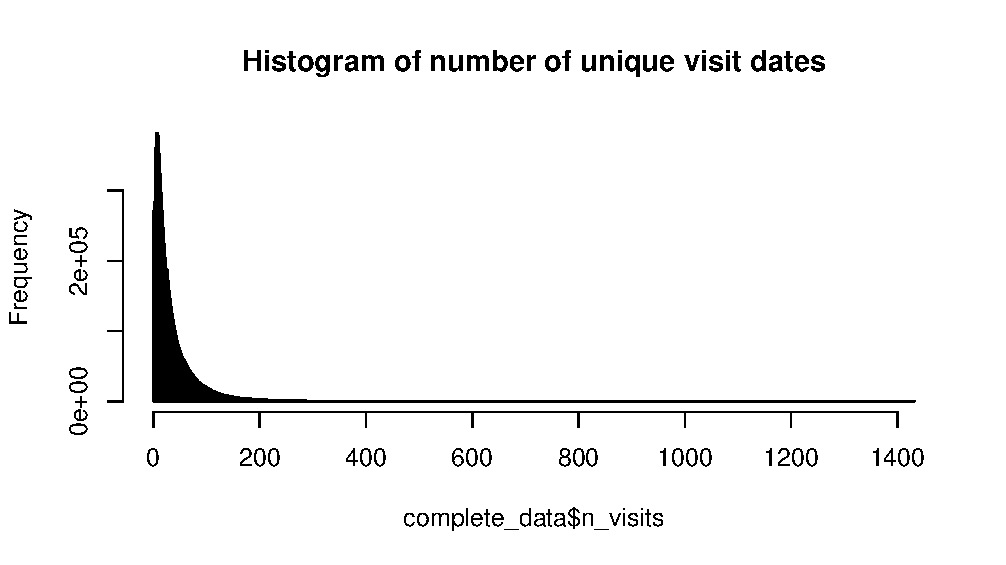
\includegraphics[width=.7\textwidth]{nvisits_hist.pdf}
\end{center}

The median control has 22 visits, while the median case has 33 visits.

Proportion of observed Charlson scores plotted against number of visits, separating controls (black) and cases (red):

\begin{center}
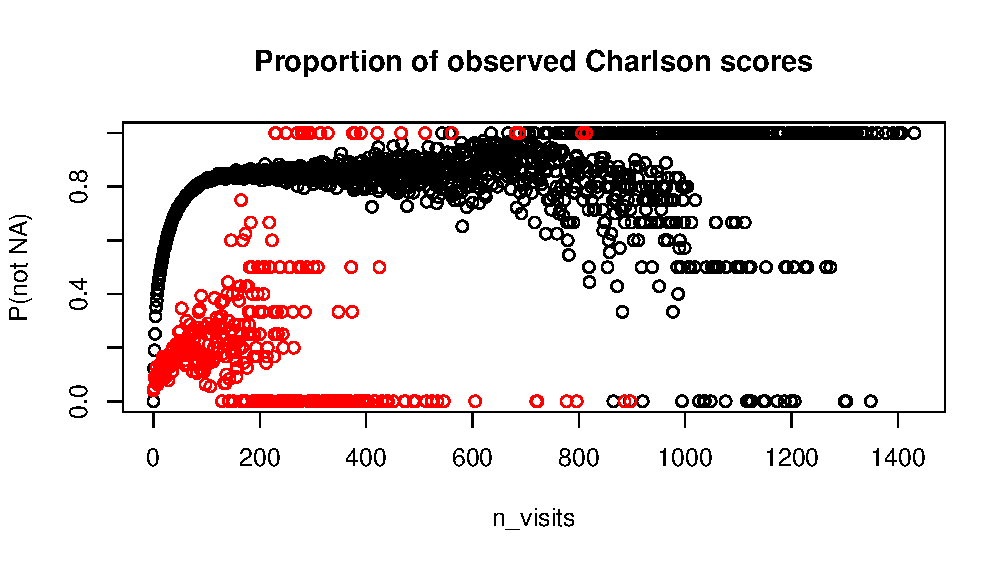
\includegraphics[width=.6\textwidth]{nvisits_scatter.pdf}
\end{center}

The same plot restricted to $\leq 200$ visits.
%Sample sizes are reasonably high (cases have a mean of 55 patients at each level of n\_visits):

\begin{center}
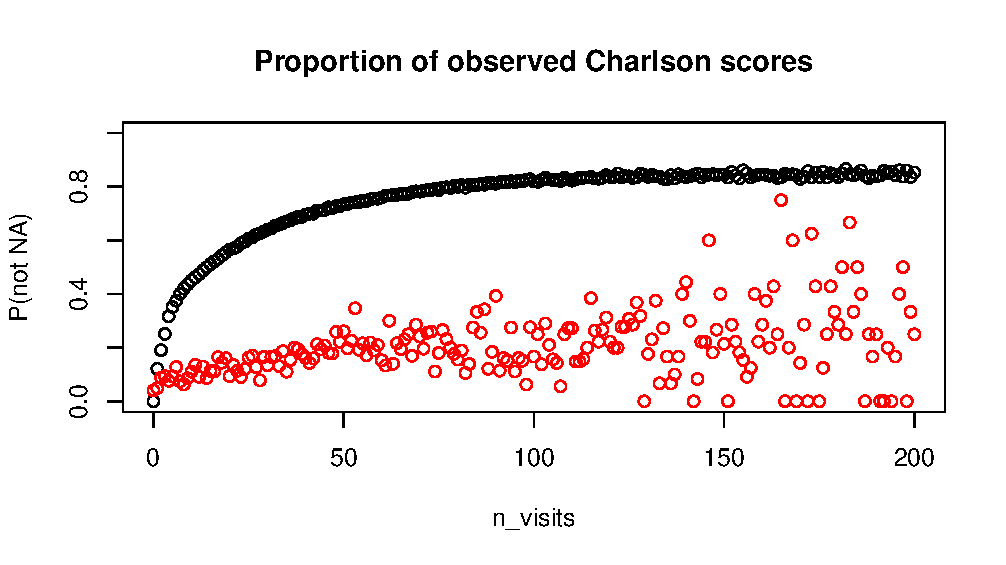
\includegraphics[width=.6\textwidth]{nvisits_scatter200.pdf}
\end{center}

{\bf Example: missingness of COPD.} Proportion of patients coded COPD=1, plotted against number of visits, separating controls (black) and cases (red):

\begin{center}
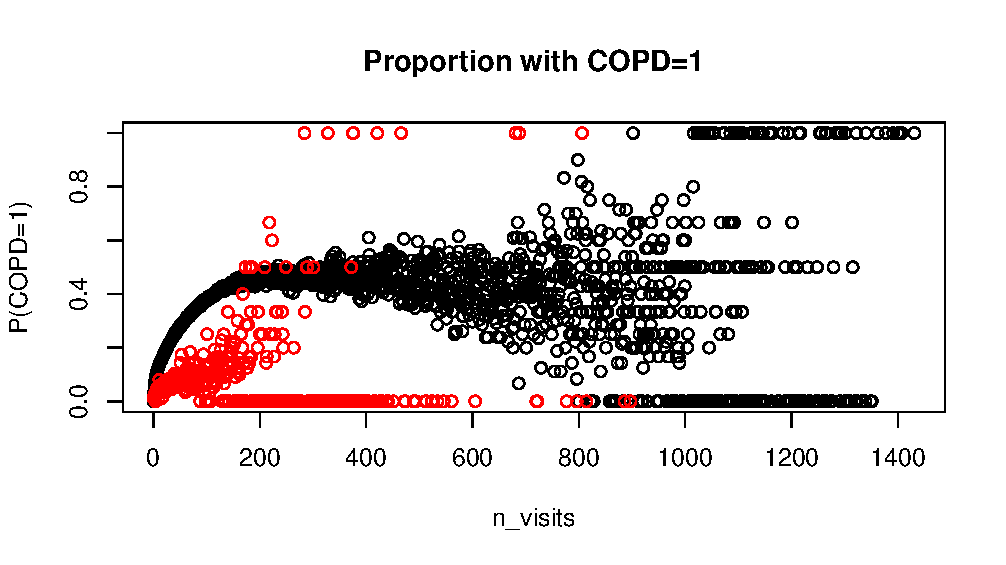
\includegraphics[width=.6\textwidth]{nvisits_scatterCOPD.pdf}
\end{center}

The same plot restricted to $\leq 200$ visits. The blue line is a model-based estimate of \\ $\mathbb{P}(\text{COPD}=1 | \text{n\_visits})$ using pooled case and control data.

\begin{center}
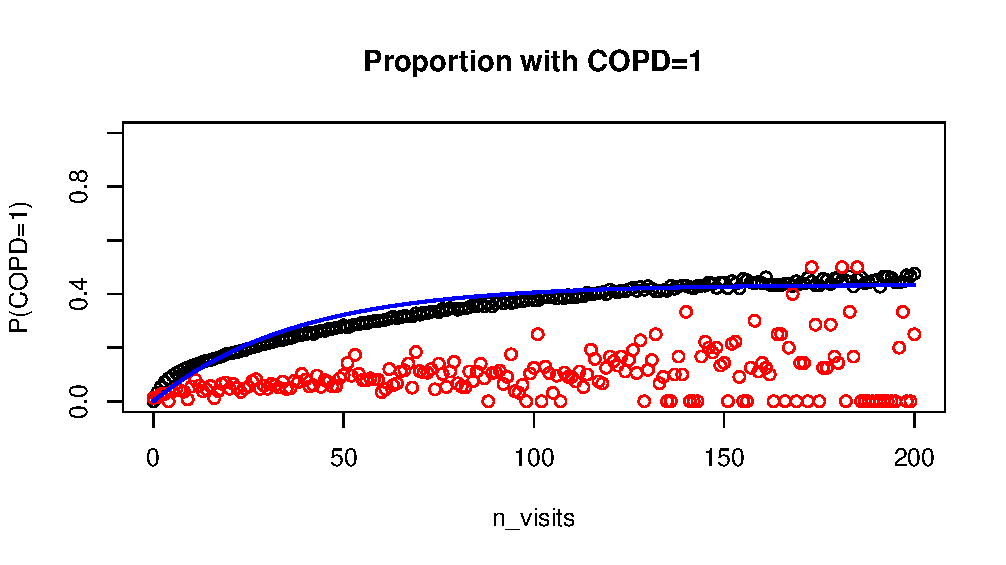
\includegraphics[width=.6\textwidth]{nvisits_scatterCOPD200.pdf}
\end{center}

For cases only, created a new COPD indicator based on the `alldxscx' table. For ICD9, 1 means you have a code `49x', for ICD10, 1 means you have a code starting with 'J44'.

Cross-classification of old and new indicator for total of 11,395 cases (overall proportions in parentheses).

\begin{center}
\begin{tabular}{|l|l|l|}
\hline
 & New COPD=1 & New COPD=0/NA \\ \hline
 Old COPD=1 & 7845 (0.688) & 2791 (0.245) \\ \hline
 New COPD=0/NA & 160 (0.014) & 599 (0.053) \\ \hline
\end{tabular}
\end{center}

Proportion of patients with COPD=1 plotted against number of visits, restricted to $\leq 200$ visits, with the old indicator in red and the new indicator in blue.

\begin{center}
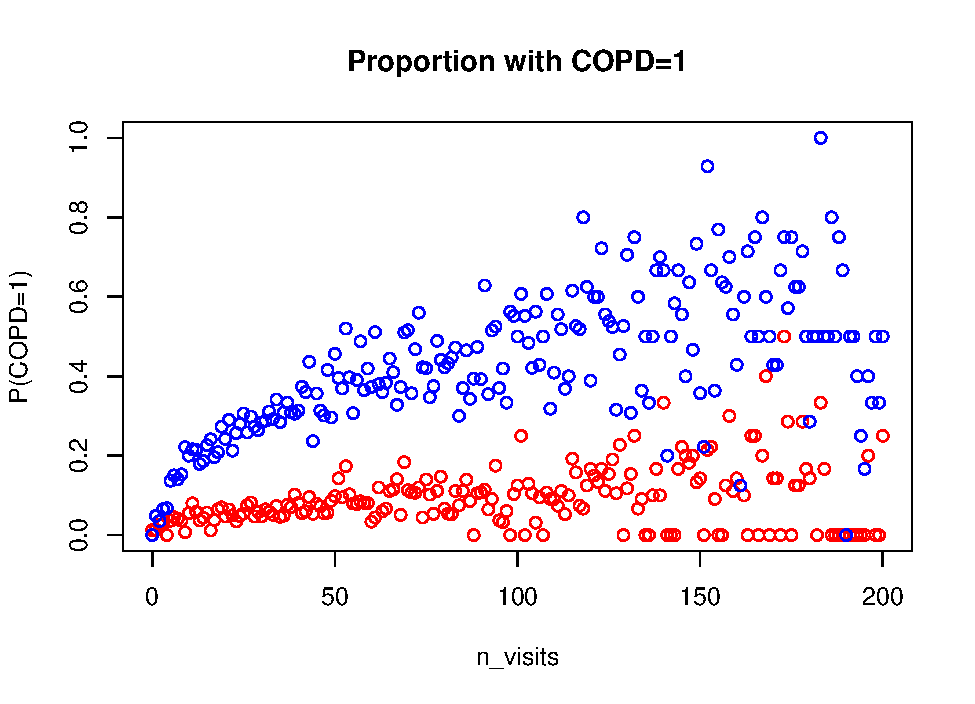
\includegraphics[width=.6\textwidth]{nvisits_scatternewCOPD200.pdf}
\end{center}

{\bf Next steps:} similarly code a new indicator for controls, see if it changes results. Generalize to other Charlson inputs (or other entirely new ICD codes), and look at ways to impute by incorporating n\_visits.

\pagebreak

Sample sizes for controls and cases for calculating the proportions in the above plots.

\begin{center}
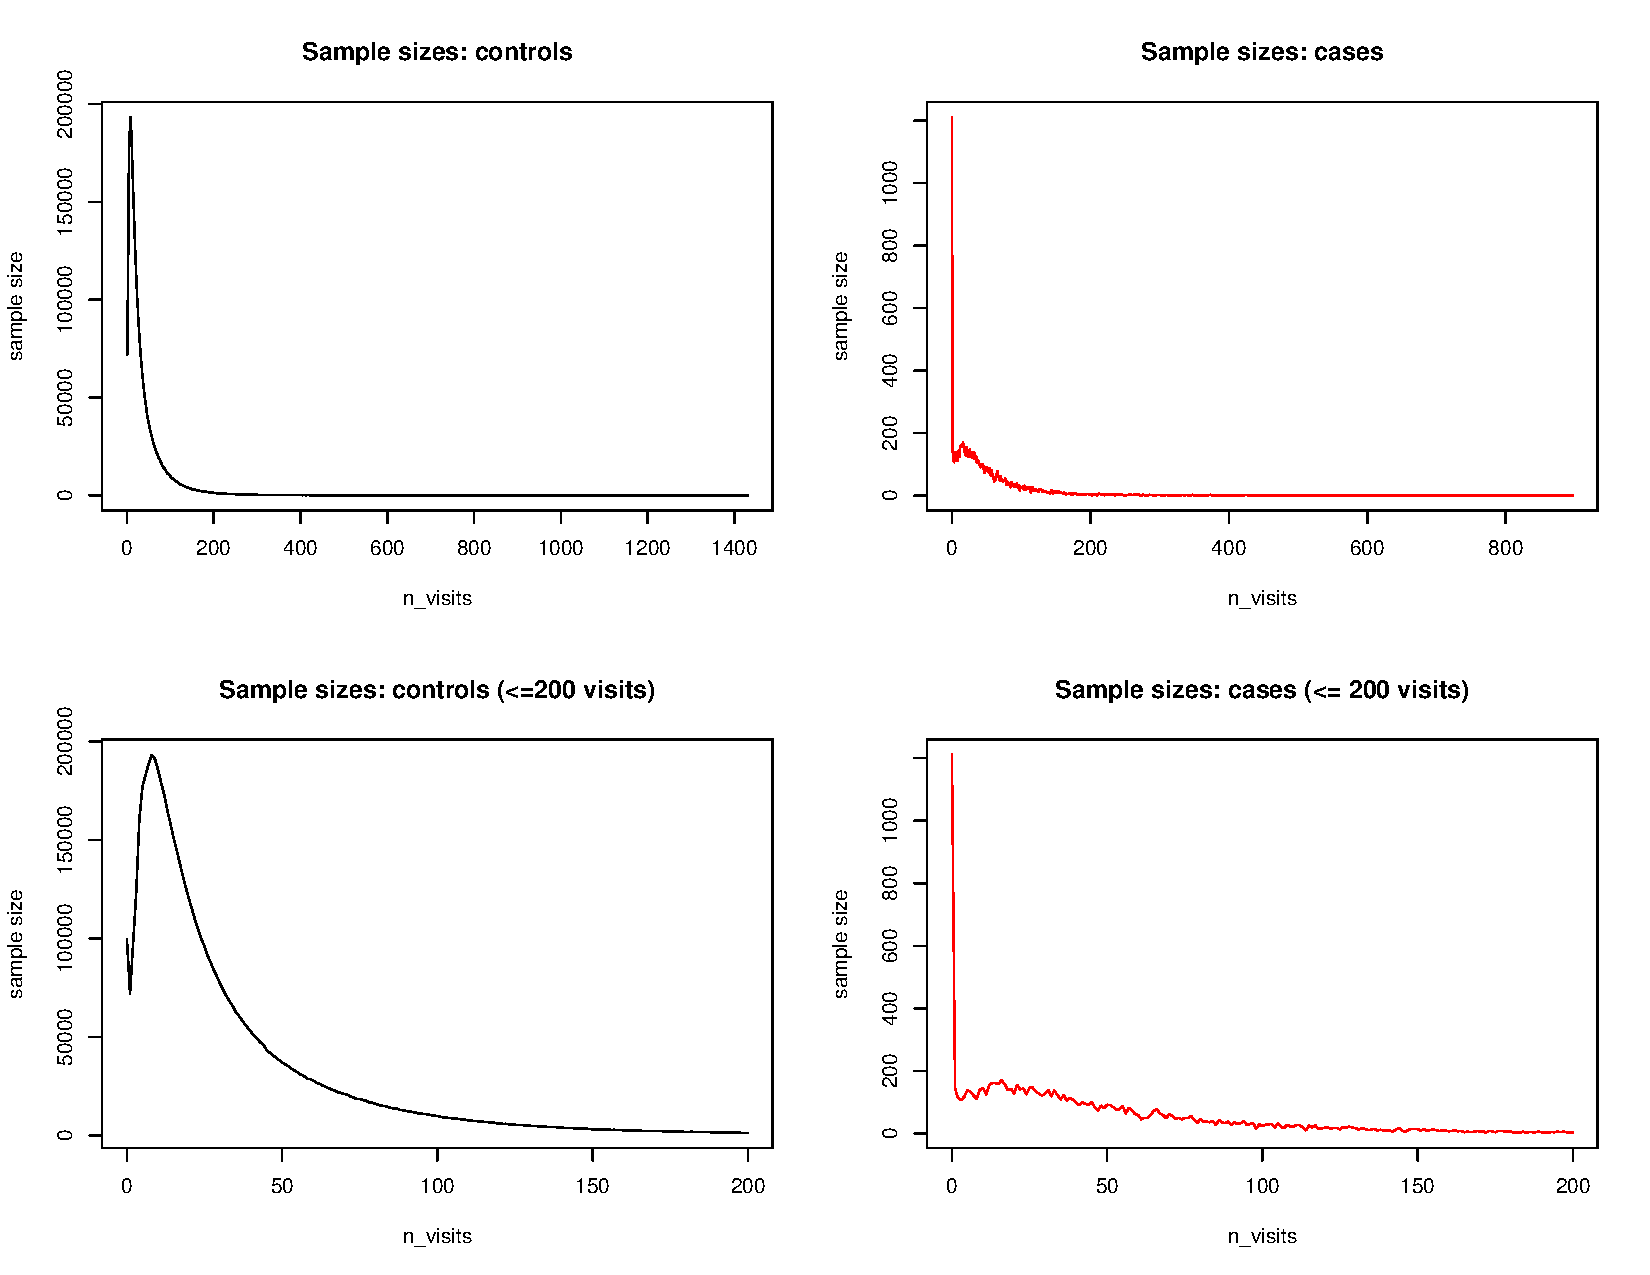
\includegraphics[width=\textwidth]{nvisits_samplesize.pdf}
\end{center}

\pagebreak
\subsubsection*{09/28 update}

\begin{itemize}
	\item Implemented new train/valid/test scheme
	\begin{itemize}
		\item Imputed records results are not exactly comparable
		\item Complete records results are comparable
	\end{itemize}
	\item Experimentation with regression imputation
	\item Experimentation with \texttt{xgboost} tuning parameters
	\item Currently working on multiple random sample with new train/valid/test scheme
\end{itemize}

\begin{table}[ht]
\centering
\begin{tabular}{lccc}
  \toprule
 & \textbf{Training AUC} & \textbf{Test AUC} & \textbf{Test AUC} \\
\textbf{Imputation method}& & \textbf{(imputed records)} & \textbf{(complete records)} \\
  \midrule
Separate class & 0.985 & 0.954 & 0.621 \\ 
 & (0.985) & (0.962) & (0.582) \\ \addlinespace
Median & 0.980 & 0.939 & 0.685 \\ 
   & (0.963) & (0.911) & (0.618) \\ \addlinespace
Regression & 0.924 & 0.742 & 0.759 \\ 
   & (0.911) & (0.750) & (0.798) \\ \addlinespace
Single rand. samp. & 0.985 & 0.777 & 0.885 \\ 
   & (0.916) & (0.780) & (0.833) \\ 
   \bottomrule
\end{tabular}
   *all with \texttt{xgboost} prediction model; AUCs in parentheses 
   denote previous results.
\end{table}

\end{document}
